\newpage
\section{Math Background}
\subsection{Review of Linear Algebra}
\subsubsection{Cross Product of 3D Vectors}


\begin{figure}[!htb]
    \centering
    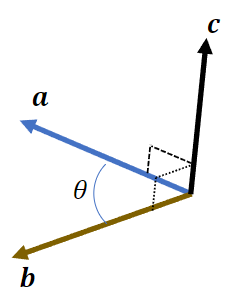
\includegraphics[width=0.12\textwidth]{pic/1052/Cross Product.png}
    \caption{Cross Product(矢量积)}
\end{figure}


\begin{align*}
    \bm{c}=\bm{a}\times\bm{b}&=\begin{bmatrix}
        a_yb_z-a_zb_y\\
        a_zb_x-a_xb_z\\
        a_xb_y-a_yb_x
    \end{bmatrix}\\
    &=\norm{\bm{a}}\norm{\bm b}\sin(\theta) \bm n\\
    \bm n &= \frac{\bm a \times \bm b}{\norm{\bm a \times \bm b}}
\end{align*}

Notice:
\begin{itemize}
    \item $\norm{\bm a \times \bm b}=\norm{\bm{a}}\norm{\bm b}\sin\theta$ 表示由$\bm a$和$\bm b$构成的平行四边形的面积
    \item If $\bm c \parallel  \bm a$, and $\bm c \ne \bm 0, \bm a \ne \bm 0$, then $\bm c \times \bm a = 0$
    \item $\bm a \times \bm b = - \bm b \times \bm a $
    \item $\bm a \times(\bm b + \bm d )=\bm a \times \bm b + \bm a \times \bm d$
    \item 矢量积没有结合律, 即 $\bm a \times(\bm b \times \bm c)\ne (\bm a \times\bm b) \times \bm c$
    \item $\bm a \times(\bm b \times \bm c)=(\bm a \cdot \bm c)\bm b - (\bm a \cdot \bm b)\bm c$
\end{itemize}

\subsubsection{Rotate a Vector}
\begin{figure}[!htb]
    \centering
    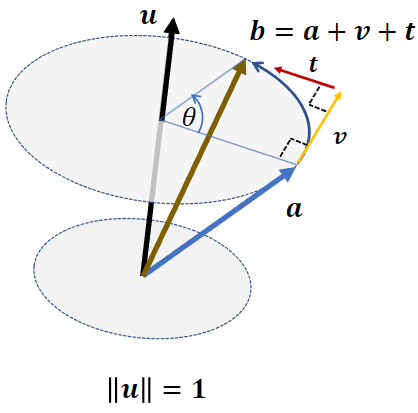
\includegraphics[width=0.22\textwidth]{pic/1052/Rotate a Vector}
    \caption{Rotate a Vector}
\end{figure}

\begin{align*}
    \bm b = \bm a + (\sin\theta)\bm u \times \bm a + (1-\cos\theta)\bm u \times(\bm u \times \bm a )
\end{align*}

\begin{proof}
    首先易知 $\bm v, \bm u$ 的方向
    \begin{align*}
        \bm v &\leftarrow \bm u \times \bm a\\
        \bm t &\leftarrow \bm u \times \bm v=\bm u \times (\bm u \times \bm a)
    \end{align*}

    然后确认 $\bm v, \bm u$ 的长度
    \begin{figure}[H]
        \centering
        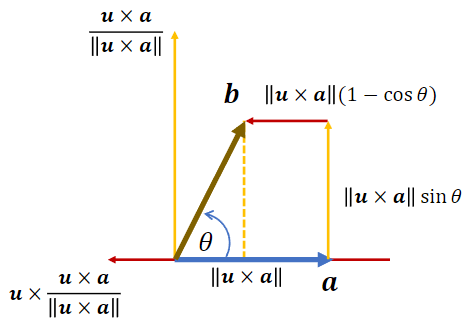
\includegraphics[width=0.309\textwidth]{pic/1052/uv.png}
        \caption{$\bm v, \bm u$}
    \end{figure}
    这里, 较长的黄线与红线表示两个单位向量. $\bm a, \bm b$ 长度相同, 是原本的 $\bm a$ 投影到此平面的长度, $\norm{\bm a}\sin \phi =\norm{\bm u \times \bm a}$. 

    最后计算出完整的 $\bm v, \bm u$
    \begin{align*}
        \bm v &=(\sin\theta) \bm u \times \bm a\\
        \bm t &=(1-\cos\theta)\bm u \times (\bm u \times \bm a)
    \end{align*}
    
    带入 $\bm b = \bm a +\bm v +\bm t$ 即可.
\end{proof}

\subsubsection{Matrix Form of Cross Product}\label{subsub:Matrix Form of Cross Product}
对于向量 $\bm a=\begin{bmatrix}
    a_1\\ a_2\\ a_3
\end{bmatrix}, \bm b=\begin{bmatrix}
    b_1\\ b_2\\ b_3
\end{bmatrix}$, 有
\begin{align*}
    [\bm a]_{\times} = \begin{bmatrix}
        0 & - a_3 & a_2 \\
        a_3 & 0  & -a_1 \\
        -a_2 & a_1 & 0
    \end{bmatrix}
\end{align*}
称为 skew-symmetric matrix(反对称矩阵). 且 
\begin{itemize}
    \item $[\bm a]_{\times}+ [\bm a]_{\times}^\top = \bm 0$
    \item $\bm a \times \bm b = [\bm a ]_{\times } \bm b$.
    \item $\bm a \times(\bm b \times \bm c)=[\bm a ]_\times [\bm b]_{\times}\bm c$
    \item $\bm a \times(\bm a \times \bm c)=[\bm a ]_\times^2\bm c$
    \item $(\bm a\times \bm b)\times \bm c = [\bm a \times \bm b]_\times \bm c$
\end{itemize}

\subsubsection{Matrix Form of Rotate a Vector}

\begin{figure}[!htb]
    \centering
    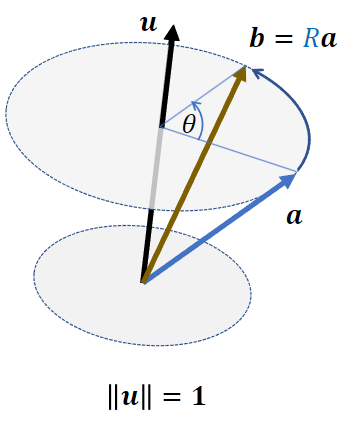
\includegraphics[width=0.309\textwidth]{pic/1052/Matrix Form of Rotate a Vector}
    \caption{Matrix Form of Rotate a Vector}
\end{figure}
Rodrigues' rotation formula:

\begin{align*}
    \bm b &= R \bm a\\
    &= \left(\bm I + (\sin\theta)[\bm u]_\times + (1-\cos\theta)[\bm u]_\times^2\right)\bm a
\end{align*}

\subsubsection{Rotation around Coordinate Axes}\label{subsub:Rotation around Coordinate Axes}
\begin{figure}[H]
    \centering
    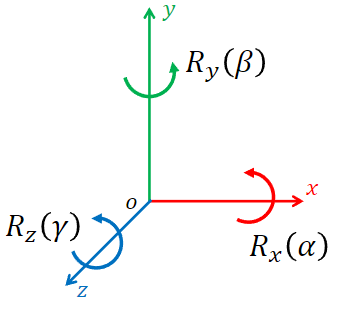
\includegraphics[width=0.22\textwidth]{pic/1052/Rotation around Coordinate Axes}
    \caption{Rotation around Coordinate Axes}
\end{figure}

Basic rotations:
\begin{align*}
    R_x(\alpha) &= \begin{pmatrix}
        1 & 0 & 0\\
        0 &\cos\alpha & - \sin \alpha\\
        0 & \sin \alpha & \cos \alpha
    \end{pmatrix}\\
    R_y(\beta) &= \begin{pmatrix}
        \cos\beta & 0 & \sin\beta\\
        0 & 1 & 0\\
        -\sin\beta & 0 & \cos\beta
    \end{pmatrix}\\
    R_z(\gamma) &= \begin{pmatrix}
        \cos\gamma & - \sin \gamma & 0 \\
        \sin \gamma & \cos \gamma & 0 \\
        0 & 0 & 1
    \end{pmatrix}\\
\end{align*}

\subsubsection{Rotation Axis and Angle}
Rotation matrix $R$ can be considered as a rotation around axis $\bm u$ by some angle $\theta$.
\begin{figure}[!htb]
    \centering
    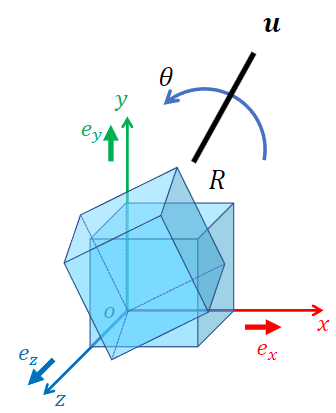
\includegraphics[width=0.22\textwidth]{pic/1052/Rotation Axis and Angle}
    \caption{Rotation Axis and Angle}
\end{figure}

To find axis $\bm u$ and angle $\theta$,
\begin{align*}
    R\bm u = \bm u &= R^\top \bm u \\
    (R-R^\top)\bm u &= 0\\
    \begin{bmatrix}
        0 & -(r_{21}-r_{12}) & r_{13}-r_{31}\\
        r_{21}-r_{12} & 0 & -(r_{32}-r_{23})\\
        -(r_{13}-r_{31}) & r_{32}-r_{23} & 0
    \end{bmatrix}\bm u &=0\\
    \bm u'\times \bm u &=0\\
    \therefore\ \bm u \leftarrow \bm u' =\begin{bmatrix}
        r_{32}-r_{23} \\
        r_{13}-r_{31} \\
        r_{21}-r_{12}
    \end{bmatrix} &\leftarrow R-R^\top\\
    \norm{\bm u'}&=2\sin\theta
\end{align*}
From Skew-symmetric matrix to cross product. \\
When $R\ne R^\top \iff \sin\theta \ne 0 \iff \theta\ne 0^{\circ} or 180^{\circ}$


\subsection{Representations of 3D rotation}
\subsubsection{Rotation matrices}
\begin{itemize}
    \item $R^\top R = I$
    \item $\det R=1$
    \item degrees of freedom (DoF) = 3
\end{itemize}


\subsubsection{Euler angles}
任意的旋转可以表示为三个基础旋转的组合. 基础旋转在 \ref{subsub:Rotation around Coordinate Axes} 定义.

Conventions of Euler Angles:
\begin{itemize}
    \item intrinsic rotations: axes attached to the object
    \item extrinsic rotations: axes fixed to the world
\end{itemize}

Gimbal Lock(万象锁): 当两个轴平行时, 一个自由度会被锁定.
\begin{figure}[!htb]
    \centering
    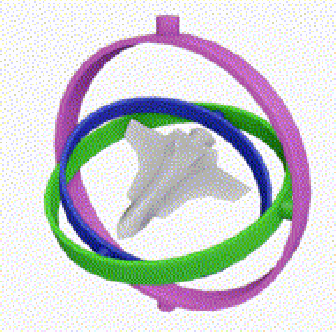
\includegraphics[width=0.22\textwidth]{pic/1052/Gimbal Lock}
    \caption{Gimbal Lock}
\end{figure}


\subsubsection{Rotation vectors/Axis angles}
\begin{itemize}
    \item Axis angle$(\bm u, \theta)$: 使用一个向量 $\bm u$ 和一个标量 $\theta$ 表示旋转.
    \item Rotation vector: $\bm \theta = \theta \bm u$. Obviously,
    \begin{align*}
        \theta = \norm{\bm \theta}\ \bm u = \frac{\bm \theta}{\norm{\bm \theta}}
    \end{align*}
\end{itemize}


\subsubsection{Quaternions(四元数)}
一个 2D 的旋转可以被表示为一个复数:
\begin{align*}
    \bm z &= a+bi = re^{\bm i \theta} \in\mathbb{C}\\
    \bm z'&= re^{\bm i (\theta + \alpha)}\\
    &=e^{\bm i \alpha}\bm z
\end{align*}

\begin{figure}[!htb]
    \centering
    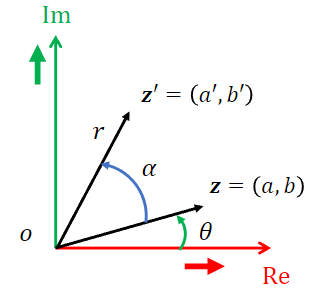
\includegraphics[width=0.22\textwidth]{pic/1052/2D rotation}
    \caption{2D rotation}
\end{figure}

\paragraph{Naive Form} 对于 3D, 扩展复数个数:
\begin{align*}
    \bm q &= a +b\bm i + c\bm j + d\bm k\in \mathbb{H}, a,b,c,d\in \mathbb{R}
\end{align*}
\begin{itemize}
    \item $\bm i^2 = \bm j^2 = \bm k^2=\bm{ijk} = -1$
    \item $\bm{ij}=\bm k, \bm{ji}=-\bm k$ 
    \item $\bm{jk}=\bm i, \bm{kj}=-\bm i$
    \item $\bm{ki}=\bm j, \bm{ik}=-\bm j$
\end{itemize}

Quaternion Arithmetic:
\begin{itemize}
    \item Conjugation(共轭): $\bm q^*=a-b\bm i - c\bm j - d\bm k$
    \item Scalar product: $t\bm q = ta +tb\bm i + tc\bm j + td\bm k$
    \item Addition: $\bm q_1 + \bm q_2= (a_1+a_2) +(b_1+b_2)\bm i + (c_1+c_2)\bm j + (d_1+d_2)\bm k$
    \item Dot product: $\bm q_1\cdot \bm q_2 = a_1a_2+b_1b_2+c_1c_2+d_1d_2$
    \item Norm: $\norm{\bm q}=\sqrt{a^2+b^2+c^2+d^2}=\sqrt{\bm q \cdot \bm q}$
\end{itemize}

Quaternion Multiplication:
\begin{align*}
    \bm q_1\bm q_2&=(a_1 +b_1\bm i + c_1\bm j + d_1\bm k)*(a_2 +b_2\bm i + c_2\bm j + d_2\bm k)
\end{align*}

\paragraph{Matrix Form} 也可以使用矩阵形式表示四元数:
\begin{align*}
    \bm q &= w +x\bm i + y\bm j + z\bm k=\begin{bmatrix}
        w\\x\\y\\z\\
    \end{bmatrix}=\begin{bmatrix}
        w\\ \bm v
    \end{bmatrix}\in\mathbb{H}, w\in\R, \bm v\in \R^3
\end{align*}
$w=\begin{bmatrix}
    w\\\bm 0
\end{bmatrix}$ called scalar quaternion, $\bm v=\begin{bmatrix}
    0\\\bm v
\end{bmatrix}$ called pure quaternion.

Quaternion Arithmetic:
\begin{itemize}
    \item Conjugation: $\bm q^*=\begin{bmatrix}
        w\\ -\bm v
    \end{bmatrix}$
    \item Scalar product: $t\bm q = \begin{bmatrix}
        tw\\ t\bm v
    \end{bmatrix}$
    \item Addition: $\bm q_1 + \bm q_2= \begin{bmatrix}
        w_1+w_2\\ \bm v_1+\bm v_2
    \end{bmatrix}$
    \item Dot product: $\bm q_1\cdot \bm q_2 = w_1w_2+\bm v_1\cdot\bm v_2$
    \item Norm: $\norm{\bm q}=\sqrt{w^2+\bm v\cdot \bm v}=\sqrt{\bm q \cdot \bm q}$
\end{itemize}

Quaternion Multiplication:
\begin{align*}
    \bm q_1\bm q_2&=\begin{bmatrix}
        w_1\\ \bm v_1
    \end{bmatrix}\begin{bmatrix}
        w_2\\ \bm v_2
    \end{bmatrix}\\
    &=\begin{bmatrix}
        w_1 & -x_1 & -y_1 & -z_1 \\
        x_1 &  w_1 & -z_1 &  y_1 \\
        y_1 & -x_1 &  w_1 &  x_1 \\
        z_1 & -y_1 &  z_1 &  w_1 \\
    \end{bmatrix}\begin{bmatrix}
        w_2\\x_2\\y_2\\z_2
    \end{bmatrix}\\
    &=\begin{bmatrix}
        w_1w_2-\bm v_1\cdot\bm v_2\\
        w_1\bm v_2+w_2\bm v_1+\bm v_1\times \bm v_2
    \end{bmatrix}
\end{align*}
类似 \ref{subsub:Matrix Form of Cross Product} 用反对称矩阵表示叉乘.

\begin{itemize}
    \item Non-Commutativity: $\bm q_1\bm q_2\ne \bm q_2\bm q_1$
    \item Associativity: $\bm q_1\bm q_2\bm q_3 =( \bm q_1\bm q_2)\bm q_3 = \bm q_1(\bm q_2\bm q_3)$
    \item Conjugation: $(\bm q_1\bm q_2)^*=\bm q_2^*\bm q_1^*$
    \item Norm: $\norm{\bm q}^2=\bm q^*\bm q=\bm q\bm q^*$
    \item Reciprocal(倒数): $\bm q\bm q^{-1}=\bm q^{-1}\bm q =1,\ \bm q^{-1}=\frac{\bm q^*}{\norm{\bm q}^2}$
\end{itemize}



\paragraph{Unit Quaternions}\quad

\begin{align*}
    \bm q=\begin{bmatrix}
        w\\ \bm v
    \end{bmatrix},\ \norm{\bm q}=1
\end{align*}

\begin{itemize}
    \item For any non-zero quaternion $\tilde{\bm q}$,
    \begin{align*}
        \bm q = \frac{\tilde{\bm q}}{\norm{\tilde{\bm q}}}
    \end{align*}
    \item Reciprocal:
    \begin{align*}
        \bm q^{-1}=\bm q^* = \begin{bmatrix}
            w \\ -\bm v
        \end{bmatrix}
    \end{align*}
    类似 $R^{-1}=R^\top$
\end{itemize}

\begin{figure}[!htb]
    \centering
    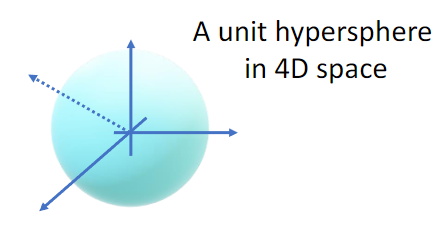
\includegraphics[width=0.22\textwidth]{pic/1052/unit quaternion}
    \caption{unit quaternion}
\end{figure}


\paragraph{Unit Quaternions as 3D Rotations} 任意3D 旋转 $(\bm v, \theta)$ 可以表示为一个 unit quaternion
\begin{align*}
    \bm q=\begin{bmatrix}
        w\\ \bm v
    \end{bmatrix}=\left[ \cos\frac{\theta}{2} ,  \bm u\sin\frac{\theta}{2} \right],\ \norm{\bm u}=1
\end{align*}
与 axis angles $(\bm u, \theta)$ 是一样的表示, 但形式不同.
\begin{itemize}
    \item Angle: $\theta = 2\arg \cos w$
    \item Axis: $\bm u =\frac{\bm v}{\norm{\bm v}}$
\end{itemize}

\begin{figure}[!htb]
    \centering
    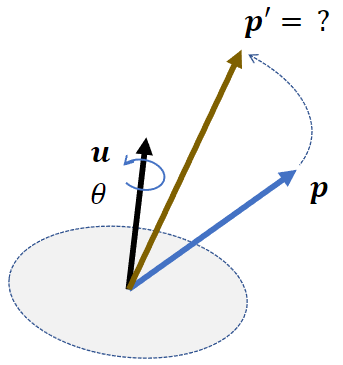
\includegraphics[width=0.22\textwidth]{pic/1052/Rotation a Vector Using Unit Quaternions}
    \caption{Rotation a Vector Using Unit Quaternions}
\end{figure}

给定 3D vector $\bm p$, 旋转结果为 $\bm p'$, 通过四元数乘积进行旋转:
\begin{align*}
    \begin{bmatrix}
        0 \\ \bm p'
    \end{bmatrix}=\bm q \begin{bmatrix}
        0\\\bm p
    \end{bmatrix} \bm q^* = (\bm q) \begin{bmatrix}
        0\\\bm p
    \end{bmatrix} (\bm q)^* 
\end{align*}
$\bm q$ 与 $-\bm q$ 表示的是同一个旋转.

对于旋转的组合, 给两个单位四元数 $\bm q_1, \bm q_2$,
\begin{align*}
    \begin{bmatrix}
        0 \\ \bm p''
    \end{bmatrix}=(\bm q_2\bm q_1)\begin{bmatrix}
        0 \\ \bm p
    \end{bmatrix}(\bm q_2\bm q_1)^*
\end{align*}

\paragraph{Interpolation}\quad
\begin{itemize}
    \item Linear Interpolation
    \begin{align*}
        {\bm q}_t &= (1-t)\bm q_0 + t\bm q_1
    \end{align*}
    $\bm q_t$ 不是单位四元数
    \item Linear Interpolation + Projection
    \begin{align*}
        \tilde{\bm q}_t &= (1-t)\bm q_0 + t\bm q_1\\
        \bm q_t &=\frac{\tilde{\bm q}_t}{\norm{\tilde{\bm q}_t}}
    \end{align*}
    旋转的速度并不是常数
    
    \begin{figure}[!htb]
        \centering
        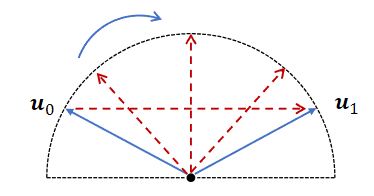
\includegraphics[width=0.309\textwidth]{pic/1052/Quaternion Interpolation}
        \caption{Linear Interpolation + Projection}
    \end{figure}
    \item SLERP: Spherical Linear Interpolation
    \begin{align*}
        \bm q_t &=\frac{\sin[(1-t)\theta]}{\sin\theta}\bm q_0 + \frac{\sin t\theta}{\sin \theta}\bm q_1\\
        \cos\theta&=\bm q_0\cdot\bm q_1
    \end{align*}
    
    \begin{figure}[!htb]
        \centering
        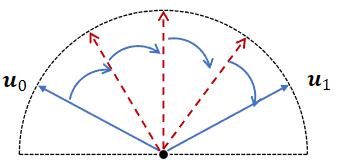
\includegraphics[width=0.309\textwidth]{pic/1052/SLERP}
        \caption{SLERP}
    \end{figure}
    \begin{proof}
        Let 
        \begin{align*}
            r = a(t)p+b(t)q
        \end{align*}
        \begin{figure}[!htb]
            \centering
            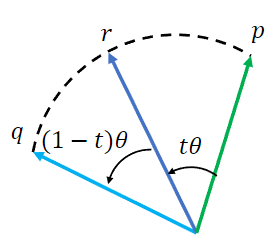
\includegraphics[width=0.22\textwidth]{pic/1052/SLERP proof.png}
            \caption{SLERP proof}
        \end{figure}
        Consider the angle $\theta$ between $p,q$: $\cos\theta=p\cdot q$

        We have
        \begin{align*}
            p\cdot r &= a(t)p\cdot p + b(t) q\cdot p\\
            \Rightarrow \cos t\theta&= a(t)+b(t)\cos\theta
        \end{align*}
        similarly
        \begin{align*}
            q\cdot r &= a(t)q\cdot p + b(t) q\cdot q\\
            \Rightarrow \cos (1-t)\theta&= a(t)\cos\theta+b(t)
        \end{align*}
        then we have
        \begin{align*}
            a(t)&=\frac{\sin[(1-t)\theta]}{\sin\theta}\\
            b(t)&=\frac{\sin t\theta}{\sin \theta}
        \end{align*}
    \end{proof}
\end{itemize}

